% !TEX root = ../main.tex

\chapter{基准分割模型3D-UNet和分割效果分析}

\section{医疗图像语义分割基础}

图像的语义分割是一种像素级的分类技术,输入一张(RGB彩色或灰度)图片,分类器输出图片上每一个像素所属的类别标签。基于深度
学习的图像语义分割方法,其主要算法是卷积神经网络(Convolutional Neural Network, CNN)。卷积神经网络通常包含以下四层:
\begin{itemize}
    \item 卷积层 Convolution layer
    \item 归一化层 Normalization layer
    \item 激活函数层 Activation function
    \item 池化层 Pooling layer
\end{itemize}
CNN的基本网络结构如图\ref{fig:CNN_basic_structure}所示:
\begin{figure}[!htp]
    \centering
    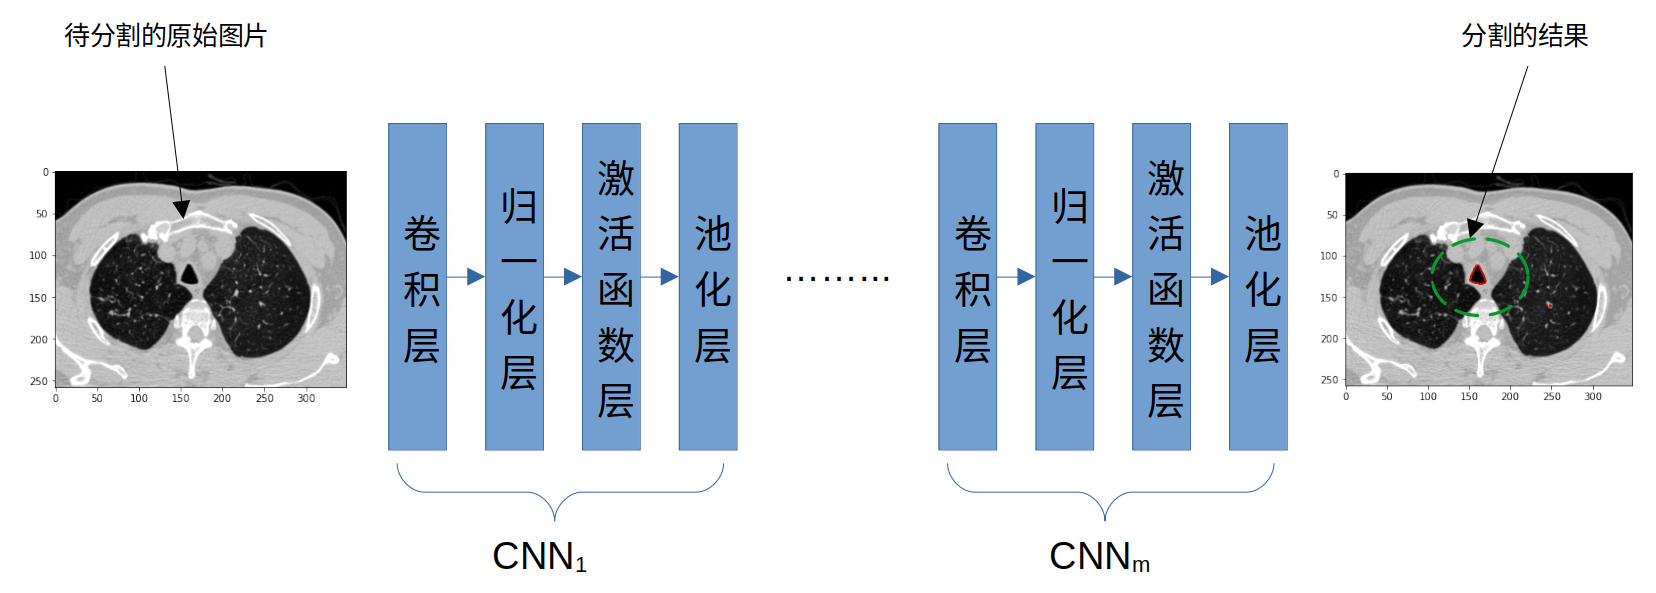
\includegraphics[width=\textwidth]{CNN_Structure}
    \bicaption[卷积神经网络基本构成]
        {卷积神经网络基本构成}
        {The basic structure of CNN}
    \label{fig:CNN_basic_structure}
\end{figure}

\noindent{}待分割的原始图片经过一层或连续多层的卷积网络后,图片的低层位置信息与高层语义信息等被提取出来,最后得到分割的结果。每次迭代
将预测的结果与真实的分割结果进行对比,选取一个合适的损失函数,计算损失值。然后通过梯度下降的反向传播,对卷积网络的参数---也就是
网络中每个神经元的权重Weight与偏置Bias---进行更新。循环进入下一次迭代,直到损失值不再降低趋于平缓,网络收敛,整个训练过程完成。

\subsection{卷积层}
卷积层的主要作用是提取特征,获得图像的局部信息。其工作原理是:在输入图像上滑动$H \times W = 3 \times 3$的窗口,每滑动
1个单位长度(此处滑动的长度称为步长Stride)就提取这个$3 \times 3$窗口内的像素信息,与同样尺寸的一个权重矩阵
(亦即卷积核尺寸convolution kernel size)做点积相乘并求和,得到当前位置的特征。

令$H3 \times W3$卷积核权重矩阵$W_{conv.kernel}$
\begin{equation}
    W_{conv.kernel} = \begin{bmatrix}
        w_1 & w_2 & w_3 \\
        w_4 & w_5 & w_6 \\
        w_7 & w_8 & w_9
    \end{bmatrix}
\end{equation}

CT扫描图像在$H3 \times W3$窗口内的Hounsfield unit\cite{HU2016CT}灰度\footnote{Hounsfield unit亨氏单位
是放射科医生在解释CT图像时使用的相对定量的无线电密度测量单位。CT重建时使用身体组织对辐射的吸收/衰减系数来生成灰度图像。
身体组织的物理密度与X射线束的吸收/衰减成正比。Hounsfield单位,也称为CT单位,是根据X射线束的线性衰减系数进行线性
变换计算而来的。}像素矩阵$X_{hu.gray}$
\begin{equation}
    X_{hu.gray} = \begin{bmatrix}
        x_1 & x_2 & x_3 \\
        x_4 & x_5 & x_6 \\
        x_7 & x_8 & x_9
    \end{bmatrix}
\end{equation}
则当前位置的特征$feat(X)$为
\begin{equation}\label{eq:conv}
\begin{split}
    {feat}(X) &= \sum{\left(W \cdot X\right)} + b \\
            &= \sum{\left(\begin{bmatrix}
                        w_1 & w_2 & w_3 \\
                        w_4 & w_5 & w_6 \\
                        w_7 & w_8 & w_9
                    \end{bmatrix} \cdot 
                    \begin{bmatrix}
                        x_1 & x_2 & x_3 \\
                        x_4 & x_5 & x_6 \\
                        x_7 & x_8 & x_9
                    \end{bmatrix}\right)} + b
\end{split}
\end{equation}
其中$b$为偏置参数Bias

式\ref{eq:conv}是在二维图像平面上的卷积操作,若在CT三维体数据上进行卷积运算,则卷积核尺寸扩展为$D3 \times H3 \times W3$
,相应地Hounsfield unit灰度像素矩阵也同步扩展到三维。三维卷积的操作如图\ref{fig:3D_Conv}所阐述:
\begin{figure}[!htp]
    \centering
    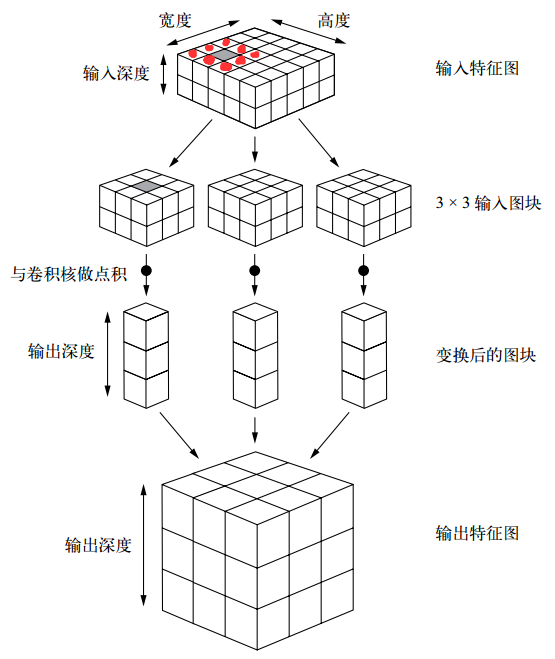
\includegraphics[width=0.5\textwidth]{Convolution_pricinple}
    \bicaption[三维卷积操作的原理]
        {三维卷积操作的原理}
        {The principle of 3D convolution}
    \label{fig:3D_Conv}
\end{figure}

\subsection{归一化层}
训练深度神经网络的计算强度非常大,训练时间漫长。减少训练时间的一种方法就是使网络中的神经元的活动归一化\cite{Ba2016LayerN}。
归一化是沿着某个指定的维度计算特征的均值与方差,对于推动深度网络收敛有着非常重要的作用。我们常用的归一化有:
\begin{enumerate}
    \item {批次归一化 Batch Normalization\cite{Ioffe2015BatchNA}}
    
    批次归一化是沿着Batch维度计算特征的均值和方差来进行归一化,批次的大小Batch size决定着预测的误差。通常取更大一些的Batch size
    有利于降低误差。过小的Batch size会导致性能下降。
    \item {层次归一化 Layer Normalization\cite{Ba2016LayerN}}
    
    层次归一化是沿着Channel维度计算特征的均值和方差来进行归一化。因为批次归一化依赖于Batch size, 尤其是不能低于mini batch size,
    而层次归一化是为了克服此问题的。
    \item {实例归一化 Instance Normalization\cite{Ulyanov2016InstanceNT}}
    
    实例归一化跟批次归一化执行相同的计算,但却是对单个样本而言。实例归一化可用于防止特定实例的均值和协方差偏移,简化学习过程。
    \item {群组归一化 Group Normalization\cite{Wu2018GroupN}}
    
    群组归一化是把Channel切分为组,在每个组内计算特征的均值和方差。群组归一化被Wu Yuxin等人\cite{Wu2018GroupN}提出来
    用于替换批次归一化,不同于层次归一化与实例归一化的方式,解决批次归一化对Batch size依赖的问题。
\end{enumerate}
我们可以用图\ref{fig:4norm}来讲解这4种归一化方式的差别。
\begin{figure}[!htp]
    \centering
    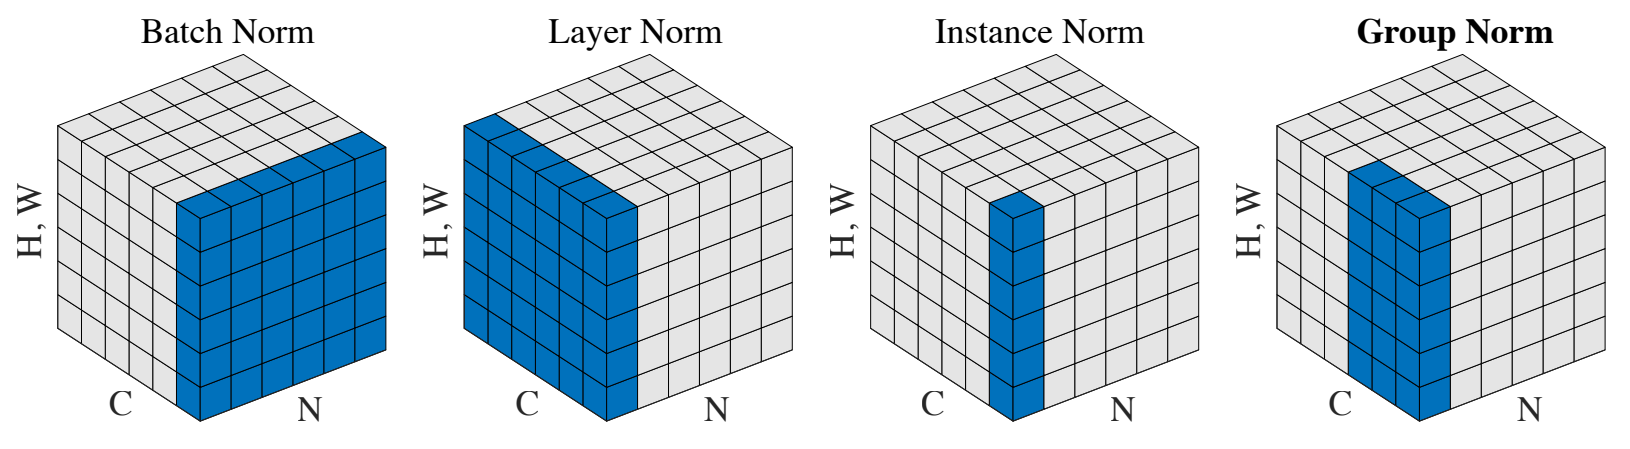
\includegraphics[width=\textwidth]{Four_Normalization_Methods}
    \bicaption[四种归一化方法的差别]
        {四种归一化方法\cite{Wu2018GroupN}}
        {Four Normalization Methods}
    \label{fig:4norm}
\end{figure}
深度网络的数据维度一般是$[Batch, Channel, Height, Width]$,简写为$[N, C, H, W]$($N$即为$Batch$)。
因为这是四个维度,我们无法画出一个四维空间的图形,所以压缩特征的$H, W$至一个维度。

\noindent{}批次归一化Batch Normalization沿Batch维度计算特征的均值和方差,归一化为$[N, H, W]$的维度,如图\ref{fig:4norm}
的Batch Norm子图的蓝色方格所示。

\noindent{}层次归一化Layer Normalization避开Batch维度,而是沿Channel维度计算特征的均值和方差,归一化为$[C, H, W]$的维度,
如图\ref{fig:4norm}的Layer Norm子图的蓝色方格所示。

\noindent{}实例归一化Instance Normalization选择单个样本计算特征的均值和方差,单个样本(也即一张图片)的维度只有$Height$
与$Weight$,所以归一化$[H, W]$的维度,如图\ref{fig:4norm}的Instance Norm子图的蓝色方格所示。

\noindent{}群组归一化Group Normalization则是介于层次归一化和实例归一化之间,其将$Channel$维度切分为很多组$Group$,
在每一个组内计算特征的均值和方差,归一化为$[C//G, H, W]$的维度,如图\ref{fig:4norm}的Group Norm子图的蓝色方格所示。

此外还有权重标准化(Weight Standardization\cite{Qiao2019WeightS})、 
批次-通道归一化(Batch-Channel Normalization\cite{Qiao2019RethinkingNA})、
深度归一化(DeepNorm\cite{Zare2017DeepNormADL})三种归一化方法,在此不做深入介绍。

\subsection{池化层}
池化的作用是缩小图像在高度和宽度方向上的空间运算,是一种降维的操作,可以用来改变当前层的输出维度,增大感受野。 池化有两种方式:
最大化池化Max Pooling和平均池化Average Pooling。最大化池化是从目标区域(图\ref{fig:pooling}的红色区域)中取出最大值,
平均池化则是计算目标区域(图\ref{fig:pooling}的深蓝色区域)的平均值。
\begin{figure}[!htp]
    \centering
    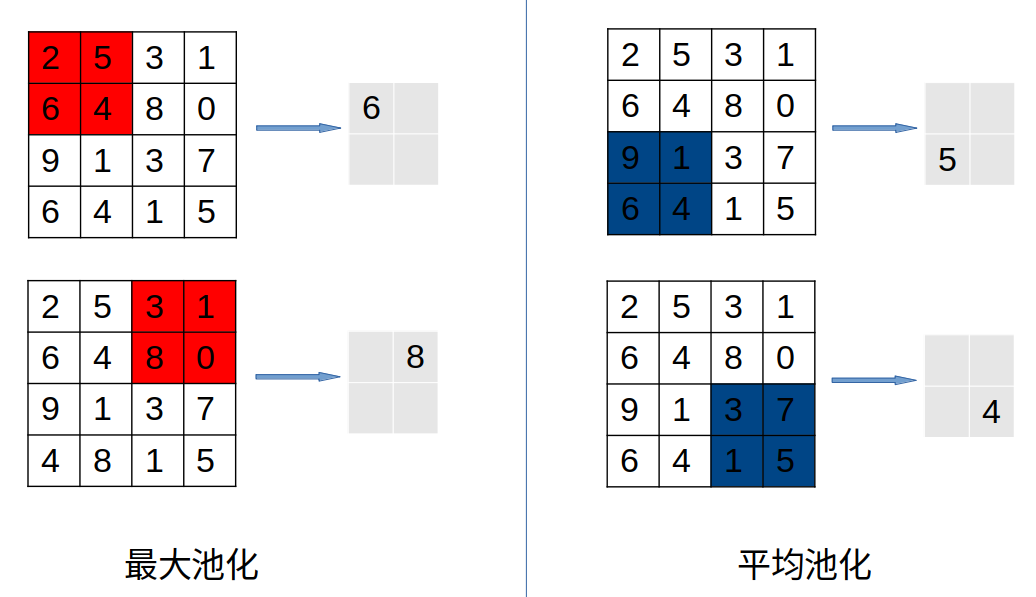
\includegraphics[width=0.7\textwidth]{Pooling}
    \bicaption[池化操作]
        {池化的基本操作}
        {The basic operations of pooling}
    \label{fig:pooling}
\end{figure}

池化层具有如下2个特征:
\begin{enumerate}
    \item {\heiti 没有要学习的参数}
    
    池化层与卷积层不一样,它没有要学习的参数。池化只是计算目标区域内的最大值或者平均值,所以不存在参数需要学习而改变。
    \item {\heiti 卷积的通道数保持不变}
    
    经过池化层,输入数据跟输出数据的通道数保持不变,是按照通道独立计算的。
    \begin{figure}[h]
        \centering
        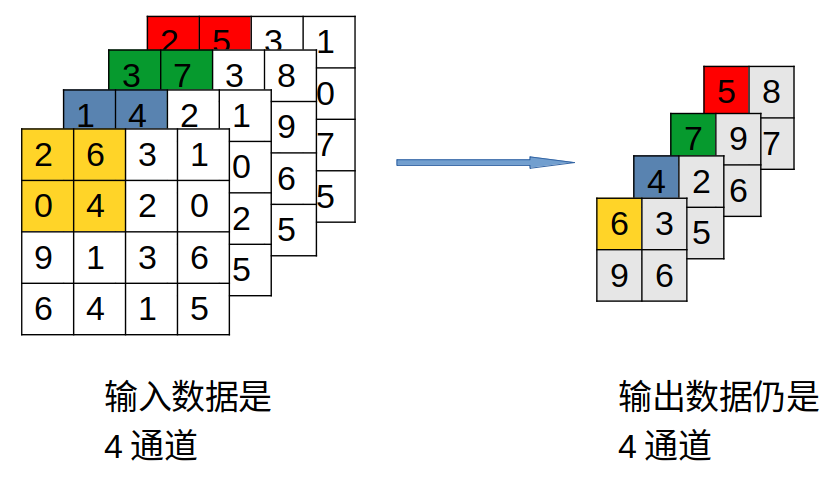
\includegraphics[scale=0.3]{Pooling_channels}
    \end{figure}
\end{enumerate}


\section{3D-UNet基准模型}
本文我们采用3D-UNet\cite{cciccek20163d}网络结构模型来分割支气管气道树,3D-UNet网络是将经典的UNet\cite{ronneberger2015u}
网络从平面图像分割扩展到三维体数据的。跟UNet网络的U型结构相似,我们将卷积层换成3D卷积,归一化层换成3D归一化,相应地池化层也更换为3D池化。
CT图像是一种体数据形式,它由一层一层的切片堆叠而成,每一层切片是一张二维的灰度图像。相比于平面图像中的像素,在CT图像中我们
定义体素Voxel为$D \times H \times W = 1 \times 1 \times 1$的立方体所含的像素,$D = 1$表明是一层切片。3D-UNet
网络的输入是$D \times H \times W$的体数据,我们称之为Cuboid,输出是每个体素的二分类分割概率图。我们在下采样路径上设计
4个卷积层块,每个卷积层块包含2层卷积。而在上采样路径上同样设计4个反卷积层块,每个反卷积层块包含2层反卷积。

\subsection{网络结构设计}

下采样路径上,每个卷积层块的结构如图\ref{fig:convblock}所示,将输入的体数据图像的通道数扩增一倍,从输入的$n$个特征通道
扩增到$2n$个特征通道。经过3D最大池化后,分辨率降低一半。
\begin{figure}[h]
    \centering
    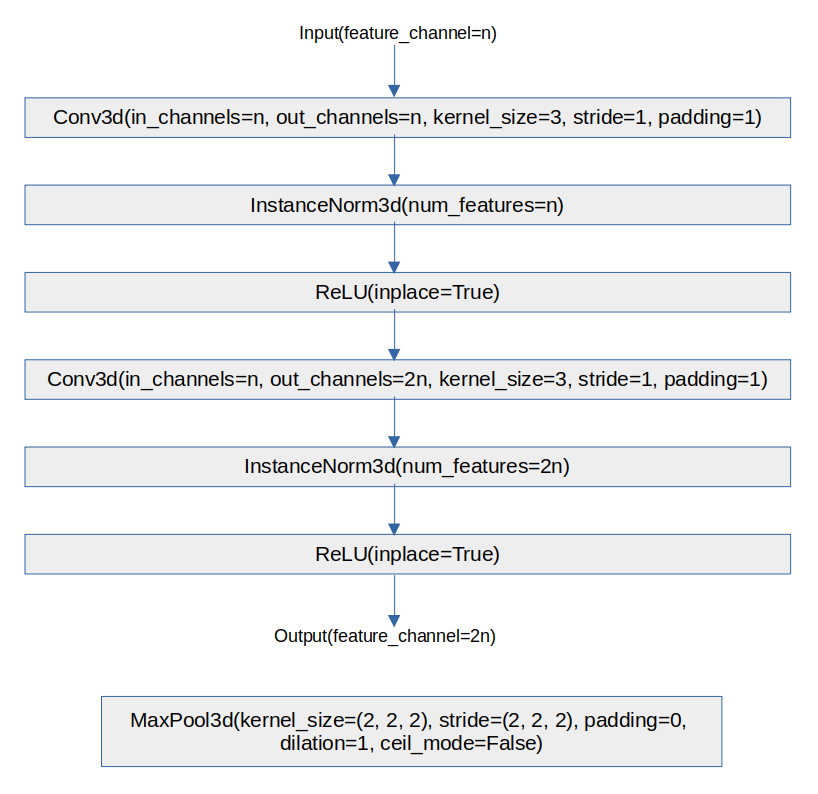
\includegraphics[width=0.8\textwidth]{Down_Conv_block}
    \bicaption[3D-UNet下采样路径上卷积层块和池化层的结构]
        {3D-UNet下采样路径上卷积层块和池化层的结构}
        {The convolution block and pooling layer in the down-sampling path of 3D-UNet}
    \label{fig:convblock}
\end{figure}

在上采样路径上,每个反卷积层块的结构如图\ref{fig:deconvblock}所示,将输入的体数据图像的通道数缩减一半。从输入的$n$个特征
通道缩减到$\frac{n}{2}$个特征通道。经过上采样池化后,分辨率升高一倍。将下采样路径降低的分辨率恢复起来,这样就实现端到端,
体素到体素的分割。
\begin{figure}[h]
    \centering
    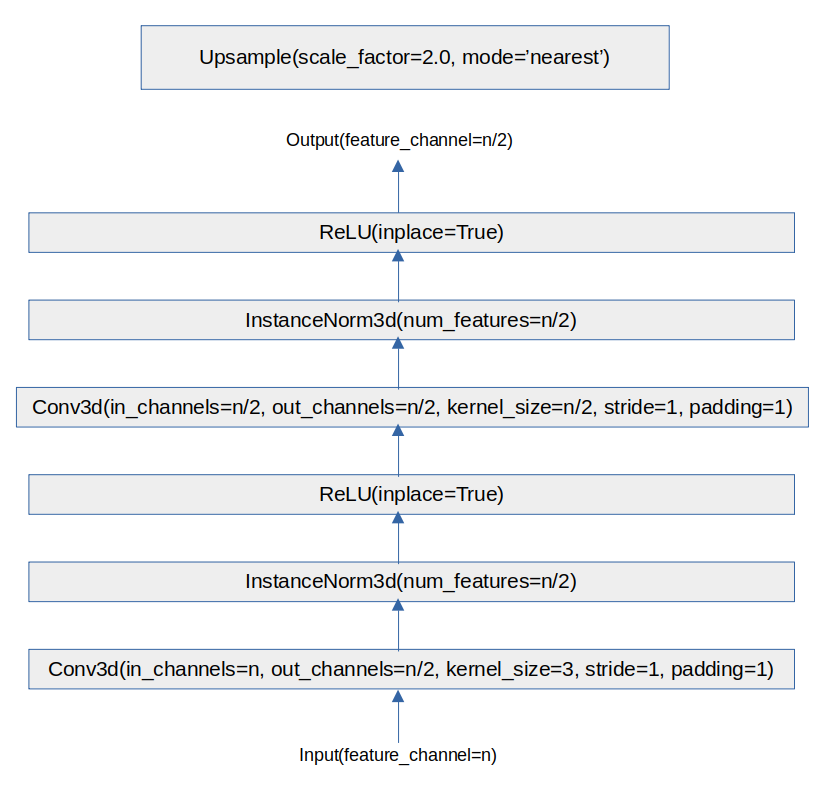
\includegraphics[width=0.8\textwidth]{Up_Conv_block}
    \bicaption[3D-UNet上采样路径上反卷积层块和池化层的结构]
        {3D-UNet上采样路径上翻卷积层块和池化层的结构}
        {The deconvolution block and pooling layer in the up-sampling path of 3D-UNet}
    \label{fig:deconvblock}
\end{figure}

我们的3D-UNet主干网络包括编码器Encoder和解码器Decoder两大部分,编码器主要用来实现图像的特征提取,扩大感受野,输出具有
类别信息的高层语义特征。解码器则逐步恢复分辨率,从而提取到低层的位置信息。更重要的是,在编码器和解码器对应的层次之间,引入
跳跃连接,将包含丰富细节信息的编码器特征拼接到解码器的高级分类特征信息中来,这样两种特征信息互相补充,最后输出每个像素的分类
概率图。我们的3D-UNet网络结构详情如图\ref{fig:3DUNetStructure}所示。由于图形宽度较大,我将其横向放置。将CT体数据(网络左侧)
\begin{figure}[ht]
    \centering
    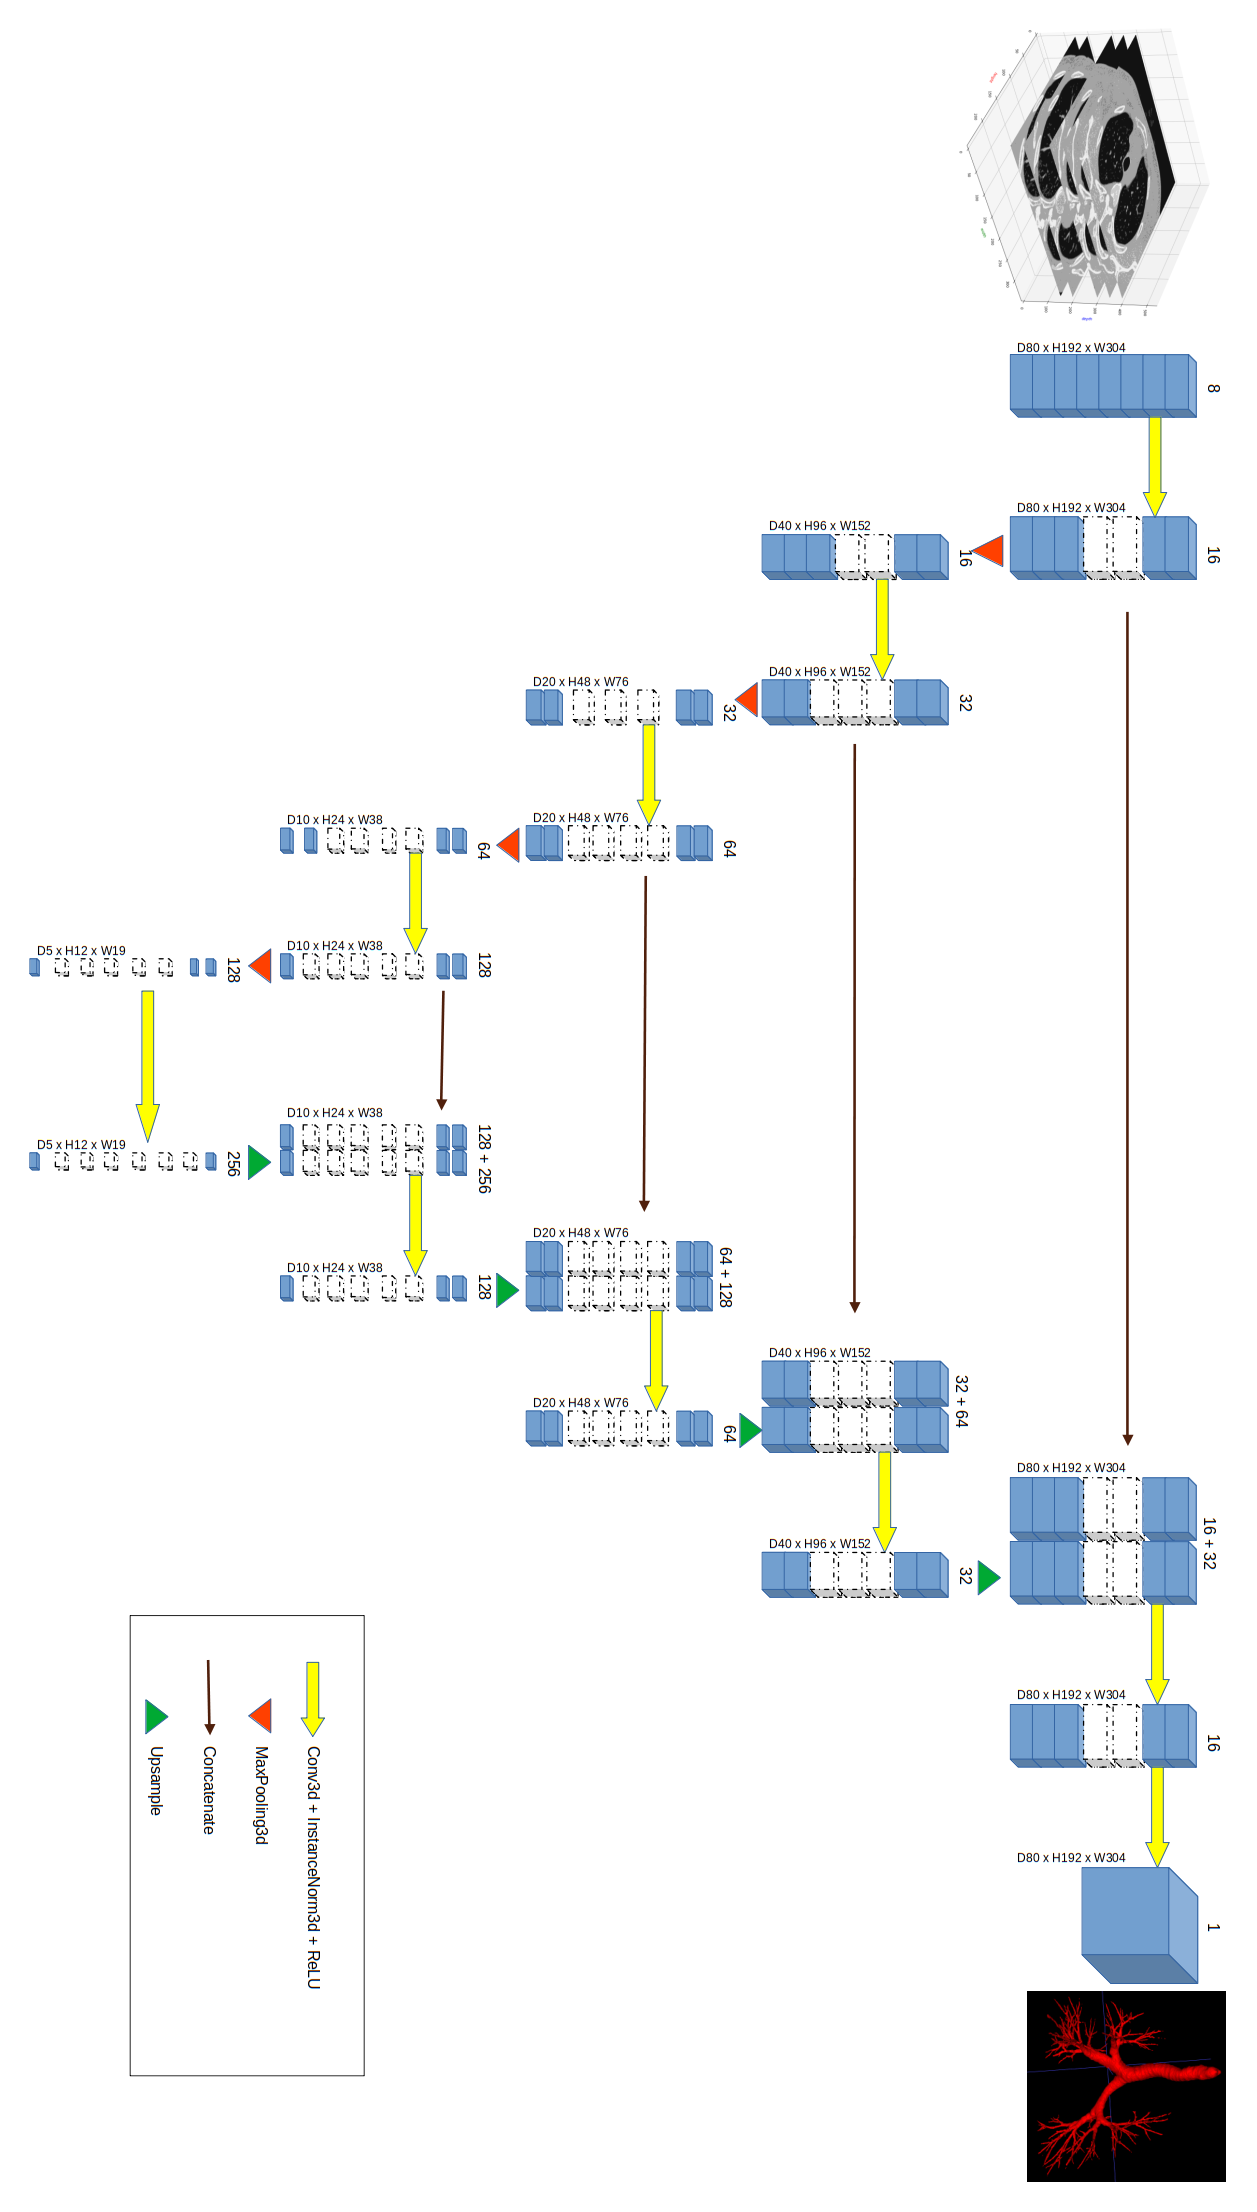
\includegraphics[height=0.72\textheight]{3DUNet_Structure_portrait}
    \bicaption[本文所设计与使用的3D-UNet网络结构]
        {本文所设计与使用的3D-UNet网络结构}
        {The 3D-UNet structure we designed in this paper}
    \label{fig:3DUNetStructure}
\end{figure}
送入网络之前,我们将其裁切为一个一个$D80 \times H192 \times W304$规格的长方体\footnote{我们将在后文讲述为什么裁切
成$D80 \times H192 \times W304$规格的。},网络学习长方体的图像特征,分割长方体内的支气管分支。训练完成后我们将属于同
一个原始CT图像的所有长方体拼接起来,最终分割出来完整的支气管气道树(网络右侧)。在长方体上面标出来的数字表示经过卷积操作后输出
的特征通道数,而在长方体侧面标注的诸如$D20 \times H48 \times W76$表示经过池化后,长方体的体积扩大或缩小,也就是长方体内
体素的分辨率增大或减小。需要指出的是,在U型结构的右侧,每一个层靠近跳跃连接的箭头处都有一个并排的长方体柱,那表示跳跃连接将
下采样路径上每一个卷积层块的特征输出拼接到上采样路径上每一个对应的反卷积层块的输入特征来。

上述的3D-UNet网络结构是本文所设计与使用,并编程实现的CT图像支气管气道树分割网络。我们将以此3D-UNet网络作为基准,通过实验
分析3D-UNet的分割结果和性能指标(包括但不限于假阳性率False Positive Rate、 真阳性率True Positive Rate、骰子相似度
系数Dice Similarity Coefficient、分支检出率Branch Detected、检测到的树长Tree Length Detected和精度等指标),提出
我们的改进方法。我们将在后面的章节展开讲述我们的改进方法,并通过实验来对比验证我们的改进方法是否有效,是否提高了分割效果和性能。

\section{数据集ATM22}
